% !TEX root = ./thesis.tex

\chapter{Evaluation}
\label{ch:eval}

Finding a definite good evaluation method for unsupervised models is a long-standing and inherent problem.


\section{Evaluation dataset}
\subsection{Data collection}

Access to large amount of training data is crucial for applying deep learning models.
Successes of deep learning on image recognition and segmentation tasks can be attributed to existence of large research datasets as ILSVRC and Places365 \cite{ILSVRC15, Zhou2016} containing millions of labeled images.
Machine translation, NLP tasks \cite{Karpathy2014, Kim2014} often rely on low-dimensional word embedding models.
Such models, as for example as word2vec or Glove \cite{Mikolov2013, pennington2014glove}, are trained on terabytes of textual data.
Deep reinforcement models might use existing gaming engines to generate required training data "on the go".
As, for example Google DeepMind team uses Atari 2D games to generate data for Q-learning \cite{Mnih2013}.

For the purpose of this research we collect visual data using the ViZDoom AI research platform \cite{Kempka2016}.
ViZDoom is a Doom-based platform for reinforcement learning.
It provides access to raw visual data from the Doom gaming engine.
Doom is a first-person shooter (FPS) computer game utilizing 3D graphics.
In context of our research the ViZDoom platform allows automatic visual data generation and collection.
Example of the output image is shown on figure \ref{fig:doom}.

We created multiple Doom maps specifically for our task using the Slade \cite{Slade3} software.
Created maps provide high diversity of textures for better discrimination between images, captured from different positions on the map.
Other reason for diverse structures on the map is to explicitly brake symmetry of the map.
Symmetric maps look alike from different player positions which leads to entangled manifolds in feature space.
Such position tend to be encoded with the same values of sparse features.
This represents a difficulty for evaluation and comparison of quality of sparse features.

We record multiple movement trajectories on each map.
More specifically, we record 10000-300000 consecutive images of unstructured movement of the player on the map for training purposes.
In addition to that, we record movement along well defined structured trajectories as a "circle" or an "eight" for model evaluation and comparison of quality of extracted features.


\begin{figure}
\centering
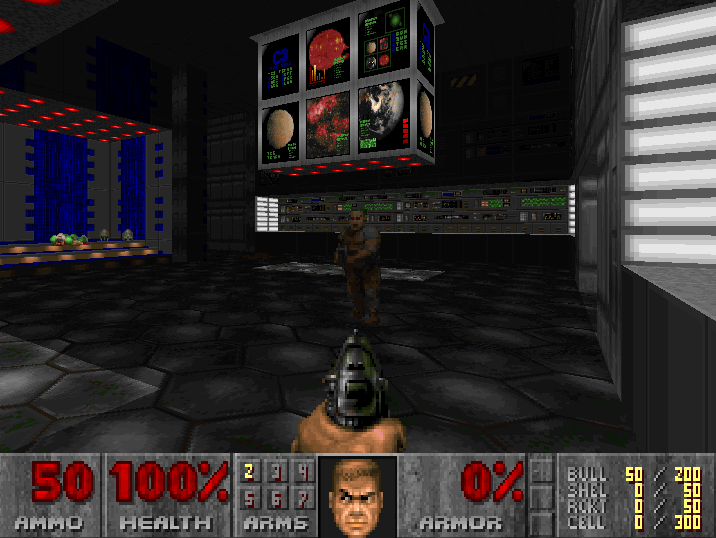
\includegraphics[width=.80\textwidth]{doom.png} %{CS0031}
\caption{Example of DoomII image collected with ViZDoom \cite{Kempka2016}.}
\label{fig:doom}
\end{figure}

\subsection{Dataset description}

We collect multiple sets of visual data with varying complexity of players movement.
We can specify next 3 classes of trajectories used either for training or evaluation:
\begin{itemize}
  \item Continuous closed trajectory without intersection. A circular movement is one example of such trajectory.
  \item Continuous closed trajectory with intersection. An \text{eight} is an example of such trajectory.
  \item Continuous random movement across the environment (map).
\end{itemize}

Furthermore, we introduce multiple complexity levels of movement across trajectories by reducing degrees of freedom of such movements:
\begin{itemize}
  \item Most restricted. Only movement along a single axis at a time is possible. This category includes movements across rectangular trajectories while maintaining fixed direction of the view or changing the direction of the view while standing still. This category provides includes trajectories of the lowest complexity.
  \item Less restricted. Multiple degrees of freedom at a time allowed. For example, movement along multiple axis facing one direction or forward movement while changing the direction of the view.
  \item Free movement across the map with no restrictions.
\end{itemize}


\subsection{Data format}

We collect RGBD images from the 3D engine. Each image has resolution of 160 by 120 pixels. Each pixel is describe by 3 color channels and a single distance channel. Each channel can take a discrete value between 0 and 255 including. This format results in 76800 dimensional inputs.

\section{Model comparison}



\subsection{Backbone model comparison}


\subsection{Regularization}


\subsection{Dataset complexity}


\subsection{Relevance of depth information}


\section{Predictive evaluation}

Describe proposed metrics and justify the usage.

\section{Loop closure detection}

Compare to \cite{Xia2016} on Freiburg2 dataset for loop closure detection.

\section{Manifold construction}

Compare to \cite{Jaderberg2015} in terms of how valuable the representation comparing to their results.

\section{Topology reconstruction}

Shall be removed(
